\chapter{Synthesis} \label{cha:synthesis} %\thispagestyle{main}

\begin{figure}[ht]
	\centering
	\resizebox{\textwidth}{!}{
		%\begin{tikzpicture}
%	[outer sep=0,
%>=latex,
%align=center]
%% Draw nodes
%\node[place]		(human_in)	[draw=none]											{Control\\input};
%\node[place]		(embed)		[inner sep=1mm,rectangle,right=10mm of human_in]	{Control\\system};
%\node[place]		(wave_gen)		[inner sep=1mm,rectangle,right=5mm of embed]			{Pulse\\generator};
%\node[place]		(pwr_stg)	[inner sep=1mm,rectangle,right=5mm of wave_gen]	{Power\\stage};
%\node[place]		(tr_switch)	[inner sep=1mm,rectangle,right=5mm of pwr_stg]	{T/R\\switch};
%\node[place]		(transducer)		[inner sep=1mm,rectangle,right=5mm of tr_switch]	{Transducer};
%\node[place]		(preamp)		[inner sep=1mm,rectangle,below=5mm of tr_switch]	{Preamplifier};
%\node[place]		(bpf)		[inner sep=1mm,rectangle,below=5mm of preamp]	{BPF};
%\node[place]		(demod)		[inner sep=1mm,rectangle,left=10mm of bpf]		{Demodulator};
%\node[place]		(lpf1)		[inner sep=1mm,rectangle,above=5mm of demod]		{LPF 1};
%\node[place]		(lpf2)		[inner sep=1mm,rectangle,below=5mm of demod]		{LPF 2};
%\node[place]		(sha1)		[inner sep=1mm,rectangle,left=5mm of lpf1]		{SHA 1};
%\node[place]		(sha2)		[inner sep=1mm,rectangle,left=15mm of lpf1]		{SHA 2};
%
%% Draw lines between nodes
%\draw [|->] 		(human_in) 		to 		(embed);
%\draw [->]			(embed)			to		(wave_gen);
%\draw [->]			(wave_gen)		to		(pwr_stg);
%\draw [->]			(pwr_stg)		to		(tr_switch);
%\draw [<->]			(tr_switch)		to		(transducer);
%\draw [->]			(tr_switch)		to		(preamp);
%\draw [->]			(preamp)		to		(bpf);
%\draw [->]			(bpf)		to		(demod);
%\draw [->]			(demod)		to		(lpf1);
%\draw [->]			(demod)		to		(lpf2);
%\draw [-|>]			(lpf1)		to		(sha1);
%\draw [-|>]			(lpf2)		to		(sha2);
%\draw [-|>]			(sha1)		to		(embed);
%\draw [-|>]			(sha2)		to		(embed);
%
%% Draw rectangle
%\draw[draw=black,dashed,red] (13mm,8mm) rectangle ++(45mm,-15mm);
%\end{tikzpicture}
%\begin{tikzpicture}
%	[outer sep=0,
%	>=latex,
%	align=center,
%	line width = 1pt,
%	% on grid,
%	start chain = going right,
%	node distance = 5cm,
%	%box/.style = {draw, rectangle, font=\huge, on chain},
%	box/.style = {draw, rectangle, on chain},
%	%L/.style = {draw, red, -{Stealth[scale=3,length=3,width=2]}},
%	L/.style = {draw, -{Stealth[scale=3,length=3,width=2]}},
%	%T/.style = {draw, red, rounded corners,
%		T/.style = {draw, rounded corners,
%			to path={-| (\tikztotarget)},
%			-{Stealth[scale=3,length=3,width=2]}}]
%
%		% Draw nodes
%		\node[place]		(human_in)	[draw=none]											{Control\\input};
%		\node[place]		(embed)		[inner sep=1mm,rectangle,right=10mm of human_in]	{Control\\system};
%		\node[place]		(wave_gen)		[inner sep=1mm,rectangle,right=5mm of embed]			{Pulse\\generator};
%		\node[place]		(pwr_stg)	[inner sep=1mm,rectangle,right=5mm of wave_gen]	{Power\\stage};
%		\node[place]		(tr_switch)	[inner sep=1mm,rectangle,right=5mm of pwr_stg]	{T/R\\switch};
%		\node[place]		(transducer)		[inner sep=1mm,rectangle,right=8mm of tr_switch]	{Transducer};
%		\node[place]		(preamp)		[inner sep=1mm,rectangle,below=5mm of tr_switch]	{Preamplifier};
%		\node[place]		(bpf)		[inner sep=1mm,rectangle,below=5mm of preamp]	{BPF};
%		\node[place]		(demod)		[inner sep=1mm,rectangle,left=10mm of bpf]		{Demodulator};
%		\node[place]		(lpf2)		[inner sep=1mm,rectangle,above=5mm of demod]	{LPF 2};
%		\node[place]		(lpf1)		[inner sep=1mm,rectangle,left=5mm of demod]		{LPF 1};
%		\node[place]		(sha2)		[inner sep=1mm,rectangle,left=10mm of lpf2]		{SHA 2};
%		\node[place]		(sha1)		[inner sep=1mm,rectangle,left=27.5mm of lpf2]		{SHA 1};
%
%		% Draw lines between nodes
%		\draw [L,|->] 		(human_in) 		to 		(embed);
%		\draw [L,->]			(embed)			to		(wave_gen);
%		\draw [L,->]			(wave_gen)		to		(pwr_stg);
%		\draw [L,->]			(pwr_stg)		to		(tr_switch);
%		\draw [L,<->]			(tr_switch)		to		(transducer);
%		\draw [L,->]			(tr_switch)		to		(preamp);
%		\draw [L,->]			(preamp)		to		(bpf);
%		\draw [L,->]			(bpf)		to		(demod);
%		\draw [L,->]			(demod)		to		(lpf1);
%		\draw [L,->]			(demod)		to		(lpf2);
%		\draw [T,->]			(lpf1)		to		(sha1);
%		\draw [L,->]			(lpf2)		to		(sha2);
%		\draw [T,->]			(sha1)		to		(embed);
%		\draw [T,->]			(sha2)		to		(embed);
%
%		% Draw rectangle
%		%\draw[draw=black,dashed,red] (13mm,8mm) rectangle ++(45mm,-15mm);
%	\end{tikzpicture}
\begin{tikzpicture}
	[outer sep=0,
	>=latex,
	align=center,
	line width = 1pt,
	% on grid,
	start chain = going right,
	node distance = 5cm,
	%box/.style = {draw, rectangle, font=\huge, on chain},
	box/.style = {draw, rectangle, on chain},
	%L/.style = {draw, red, -{Stealth[scale=3,length=3,width=2]}},
	L/.style = {draw, -{Stealth[scale=3,length=3,width=2]}},
	%T/.style = {draw, red, rounded corners,
		T/.style = {draw, rounded corners,
			to path={-| (\tikztotarget)},
			-{Stealth[scale=3,length=3,width=2]}}]

		% Draw nodes
		\node[place]		(human_in)	[draw=none]											{Control\\input};
		\node[place]		(embed)		[inner sep=1mm,rectangle,right=10mm of human_in]	{Control\\system};
		\node[place]		(wave_gen)		[inner sep=1mm,rectangle,right=5mm of embed]			{Pulse\\generator};
		\node[place]		(pwr_stg)	[inner sep=1mm,rectangle,right=5mm of wave_gen]	{Power\\stage};
		\node[place]		(tr_switch)	[inner sep=1mm,rectangle,right=5mm of pwr_stg]	{T/R\\switch};
		\node[place]		(transducer)		[inner sep=1mm,rectangle,right=10mm of tr_switch]	{Transducer};
		\node[place]		(preamp)		[inner sep=1mm,rectangle,below=5mm of tr_switch]	{Preamplifier};
		\node[place]		(bpf)		[inner sep=1mm,rectangle,below=5mm of preamp]	{BPF};
		\node[place]		(demod)		[inner sep=1mm,rectangle,left=5mm of bpf]		{Demodulator};
		%\node[place]		(lpf2)		[inner sep=1mm,rectangle,above=5mm of demod]	{LPF 2};
		\node[place]		(lpf1)		[inner sep=1mm,rectangle,left=5mm of demod]		{LPF};
		%\node[place]		(sha2)		[inner sep=1mm,rectangle,left=10mm of lpf2]		{SHA 2};
		\node[place]		(sha1)		[inner sep=1mm,rectangle,left=5mm of lpf1]		{SHA};
		\node[place]		(hpf)		[inner sep=1mm,rectangle,above=5mm of sha1]		{HPF};

		% Draw lines between nodes
		\draw [L,|->] 		(human_in) 		to 		(embed);
		\draw [L,->]			(embed)			to		(wave_gen);
		\draw [L,->]			(wave_gen)		to		(pwr_stg);
		\draw [L,->]			(pwr_stg)		to		(tr_switch);
		\draw [L,<->]			(tr_switch)		to		(transducer);
		\draw [L,->]			(tr_switch)		to		(preamp);
		\draw [L,->]			(preamp)		to		(bpf);
		\draw [L,->]			(bpf)		to		(demod);
		\draw [L,->]			(demod)		to		(lpf1);
		%\draw [L,->]			(demod)		to		(lpf2);
		\draw [L,->]			(lpf1)		to		(sha1);
		%\draw [L,->]			(lpf2)		to		(sha2);
		\draw [L,->]			(sha1)		to		(hpf);
		%\draw [T,->]			(sha2)		to		(embed);
		\draw [L,->]			(hpf)		to		(embed);

		% Draw rectangle
		%\draw[draw=black,dashed,red] (13mm,8mm) rectangle ++(45mm,-15mm);
	\end{tikzpicture}
	}
	\caption[Simplified overview of the system]{Simplified overview of the system with the demodulation and control system indicated with a red dashed rectangle}
	\label{fig:1_system_overview}
\end{figure}
A simplified overview of the entire system can be seen in \cref{fig:1_system_overview}. Each of the various modules will be explained during this chapter of the report. Initially, the control system will be briefly explained and the reasons for its design choice. Secondly, the signal chain in the transmitter will be outlined and how the transducer is driven by the power stage with the added protective switching circuit. Finally, the analogue front-end will be further explained with its various subcircuits for amplifying and demodulating the signal. Lastly, the design of the \gls{dsp} within the control system will be explained.

\section{Control System}
The choice of platform for the control system is a microcontroller. A microcontroller is a small computer that is built into a single \gls{ic} chip. It includes a \gls{cpu}, memory, and \gls{io} peripherals, and it is designed to perform a specific set of tasks. Microcontrollers are used in a wide range of electronic devices, including appliances, automobiles, industrial control systems, and consumer electronics. Microcontrollers are often used in applications where a small, low-power device is needed to perform simple tasks, such as controlling a motor or reading a sensor. They are usually programmed in a high-level language, such as C or C++, and they can be programmed to perform a variety of tasks, depending on the specific application. The chosen \gls{mcu} for this project is STM32F411RE, because it is sufficient for the application and sourcing limitations within the \gls{ic} supply chain. In addition, the selected development environment was Visual Studio Code with PlatformIO and Zephyr RTOS using the programming language \gls{c} and \gls{cpp}. Both are explained in the following subsections.

\subsection{Development Environment}
\begin{figure}[htbp]
	\centering
	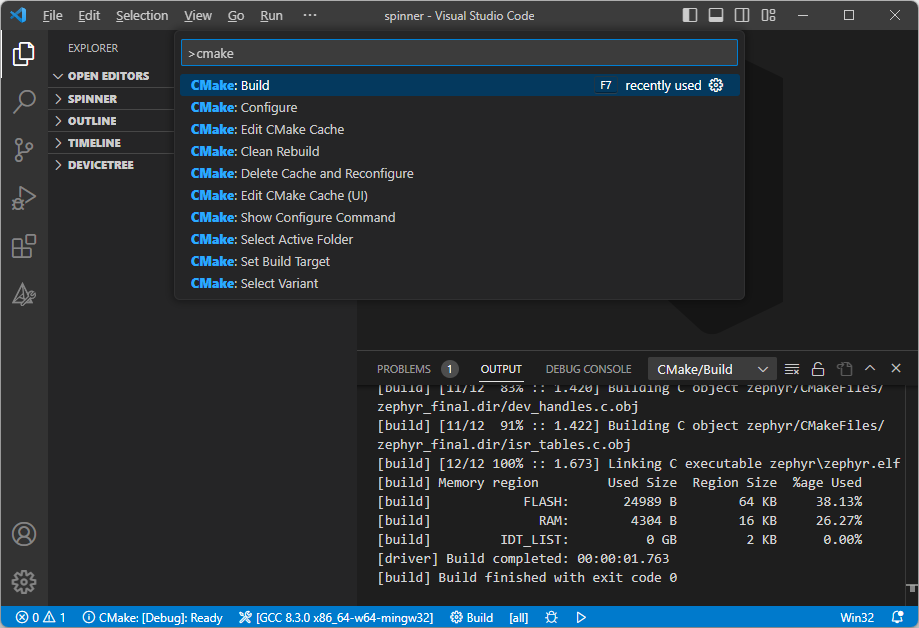
\includegraphics[width=.8\textwidth]{Figures/3_cmake_vscode.png}
	\caption[VSCode editor with CMake Tools active]{VSCode editor with CMake Tools active, displaying available tasks}
	\label{fig:3_vscode_cmake_build}
\end{figure}

Visual Studio Code (VSCode) is an \gls{open-source} code editor developed by Microsoft. It is designed to be highly customizable and efficient, with a wide range of features and extensions that allow developers to customize their workflows and improve their productivity. VSCode works in synergy with CMake through an extension. CMake is a cross-platform build system that helps developers manage the build process for their projects. It is used to generate build files for different platforms and build systems, to build projects on a wide range of platforms. When using CMake with VSCode, the basic idea is to use the CMake extension for VSCode to generate the appropriate build files for the target platform, and then use the VSCode tasks and debugging capabilities to build and debug the project. After setup of VSCode, the CMake Tools\cite{cmake} extension can be found in the VSCode Marketplace. The CMake Tools extension allows you to create, configure and build CMake projects from within VSCode. Once the extension is installed, you can create a new CMake project and configure it by specifying the path to the \texttt{CMakeLists.txt} file and other settings like the target platform and build configuration. After configuring the project, the VSCode tasks are provided to build and run the project. These tasks are defined in the \texttt{tasks.json} file, which can be customized to specify the build command and other options. Examples of tasks are build the project, cleaning the build directory, or running tests. The available CMake tasks are shown in \cref{fig:3_vscode_cmake_build}. In addition to building and running the project, VSCode allows for debugging capabilities to debug code. The CMake Tools extension provides a debug configuration template for C/C++ projects, which you can use to configure the debugger for your project. You can then set breakpoints in your code and step through it while debugging.

\subsection{Zephyr}
Zephyr is an \gls{open-source} \gls{rtos} designed for the \gls{iot}. It is a lightweight RTOS that can run on a wide range of devices, from \gls{mcu}s with as little as \qty{20}{\kilo\byte} of RAM to more powerful systems with multiple processors. Zephyr is designed to be modular and scalable, with a focus on security and low power consumption. It includes support for a wide range of hardware architectures, including ARM Cortex-M, x86, and RISC-V, and it can be used with a variety of development boards and microcontrollers. One of the key features of Zephyr is its ability to run on very small devices with limited resources. It includes support for various networking protocols, such as \gls{ble}, IPv4, and IPv6, which makes it well-suited for use in IoT applications. Zephyr is developed as part of the Linux Foundation's Zephyr Project, and it is widely used in the development of IoT and embedded systems. It is a popular choice for lightweight, flexible, and secure RTOS projects.

\subsubsection{Real-Time Operating System}
A real-time operating system is an operating system that is designed to handle real-time applications. Real-time applications are those that require timely processing of data in order to function correctly. This can include tasks such as controlling industrial machinery, monitoring and controlling processes. Real-time operating systems are designed to prioritize certain tasks and ensure that they are completed within a specific timeframe. They do this by allocating a certain amount of processing resources to each task, and by interrupting the execution of lower-priority tasks as needed to ensure that high-priority tasks are completed on time. RTOSs typically include features such as preemptive scheduling, real-time communication, and support for multiple processors and hardware architectures.

\subsubsection{Build System}
To build an application with the Zephyr kernel, you use CMake which has two phases - configuration and build. During configuration phase, CMake executes the \texttt{CMakeLists.txt} build scripts to generate an internal model of the Zephyr build. The configuration phase can be seen in \cref{fig:3_cmake_configuration}. Starting with \gls{dts}/\gls{dtsi} and then using the device tree and Kconfig to configure the set of build files for \texttt{ninja}. Once configuration is done, CMake generates build scripts that are native to the host platform using Ninja or Make. Afterwards, the generated build scripts are executed to begin the second phase, build. The build scripts can recompile the application without involving CMake after most code changes. However, in some cases, you need to execute the configuration step again before building. Zephyr uses CMake's 'target' concept to organize the build, where a target can be an executable, a library, or a generated file. The final output of the build system \texttt{ninja} is a binary file ready for \gls{flashing} using a microcontroller programmer.

\begin{figure}[htbp!]
	\centering
	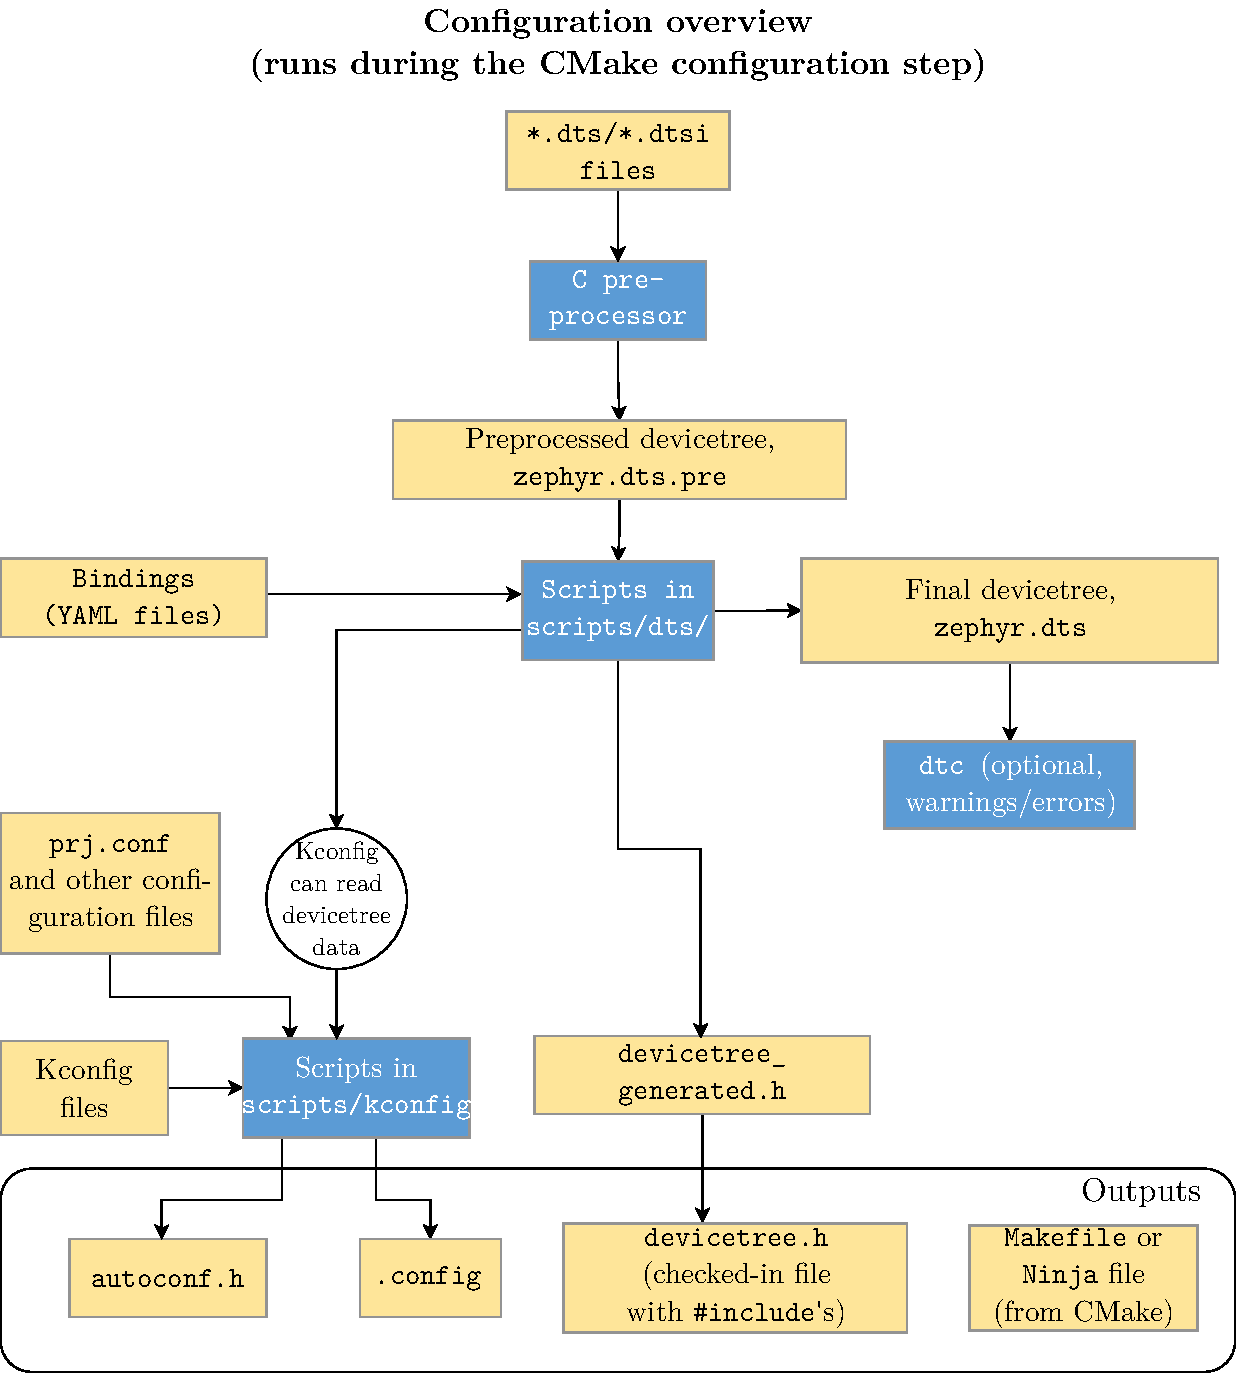
\includegraphics[width=.8\textwidth]{Figures/3_cmake_configuration.pdf}
	\caption[Configuration phase of a Zephyr application]{Configuration phase of a Zephyr application \cite{zephyrprojectdocumentation}}
	\label{fig:3_cmake_configuration}
\end{figure}
After cmake configuration phase has completed, the build phase begins. CMake invokes \texttt{ninja}, which (conceptually) has five (six, one is repeated) stages: (I) pre-build, (II) generation and compilation, (III) first-pass binary (and (IV) second-pass binary), (V) final binary and (VI) post-processing.
\begin{figure}[htbp]
	\centering
	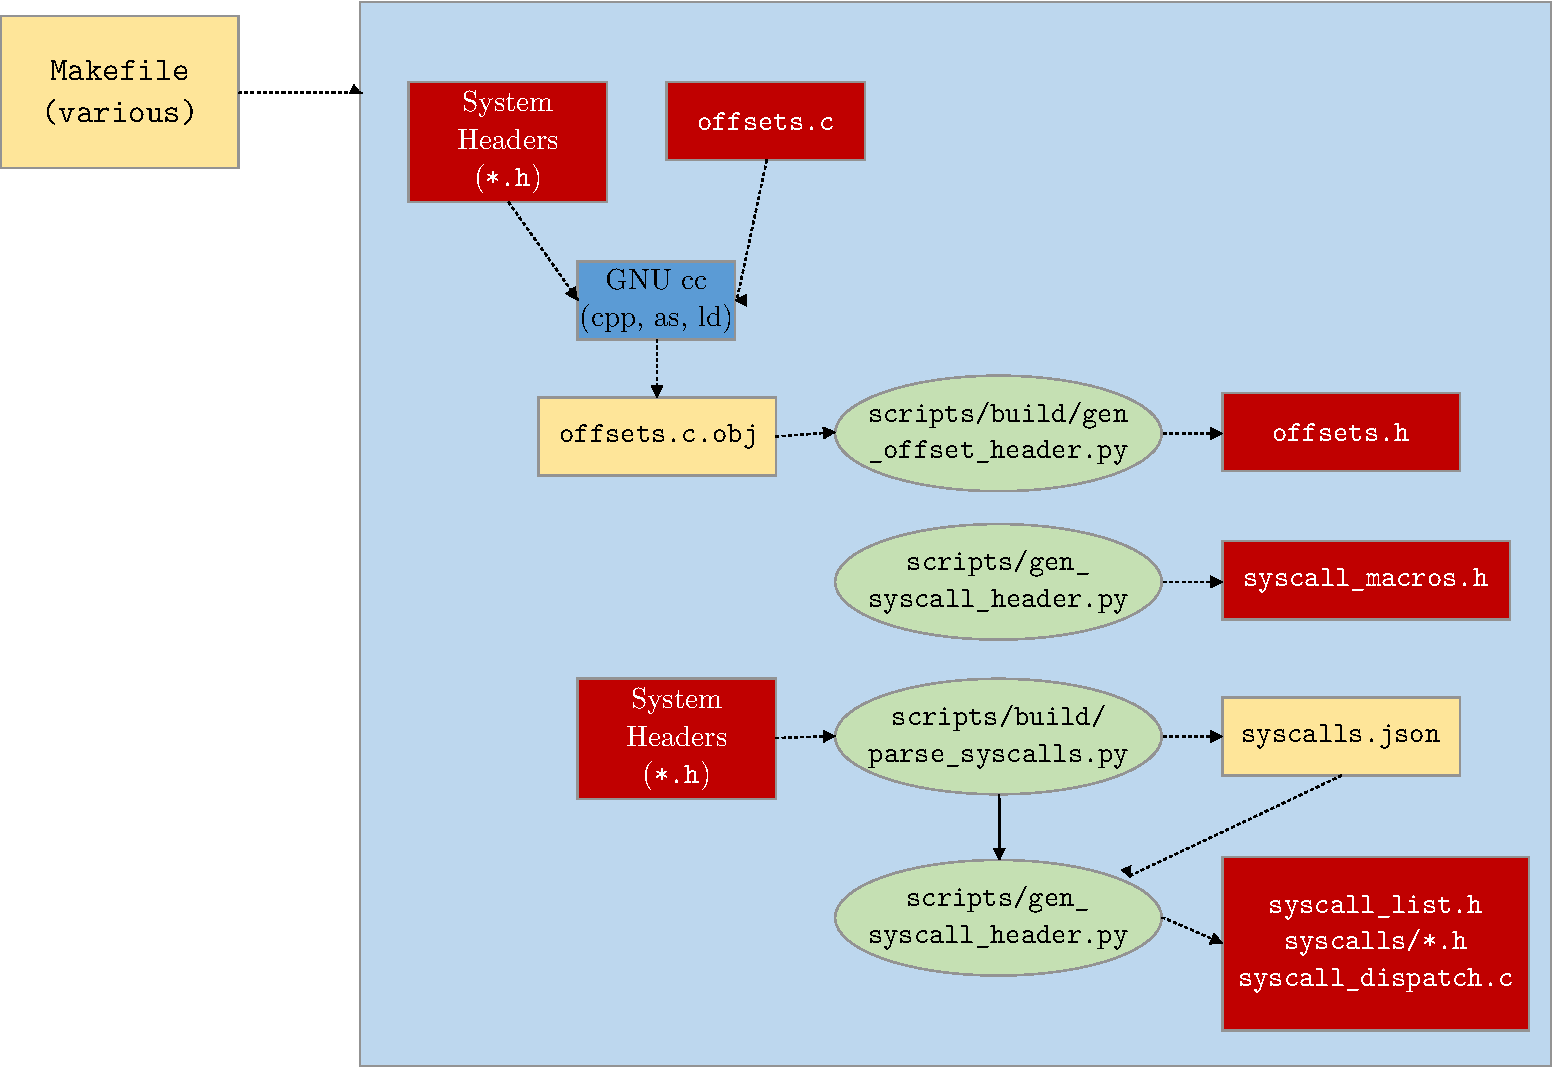
\includegraphics[width=\textwidth]{Figures/3_cmake_build1.pdf}
	\caption[Flowchart of ninja stage I, pre-build]{Flowchart of \texttt{ninja} build stage I, pre-build}
	\label{fig:3_build1}
\end{figure}
In \cref{fig:3_build1} the build system binds system call functions to implementations.
\begin{figure}[htbp]
	\centering
	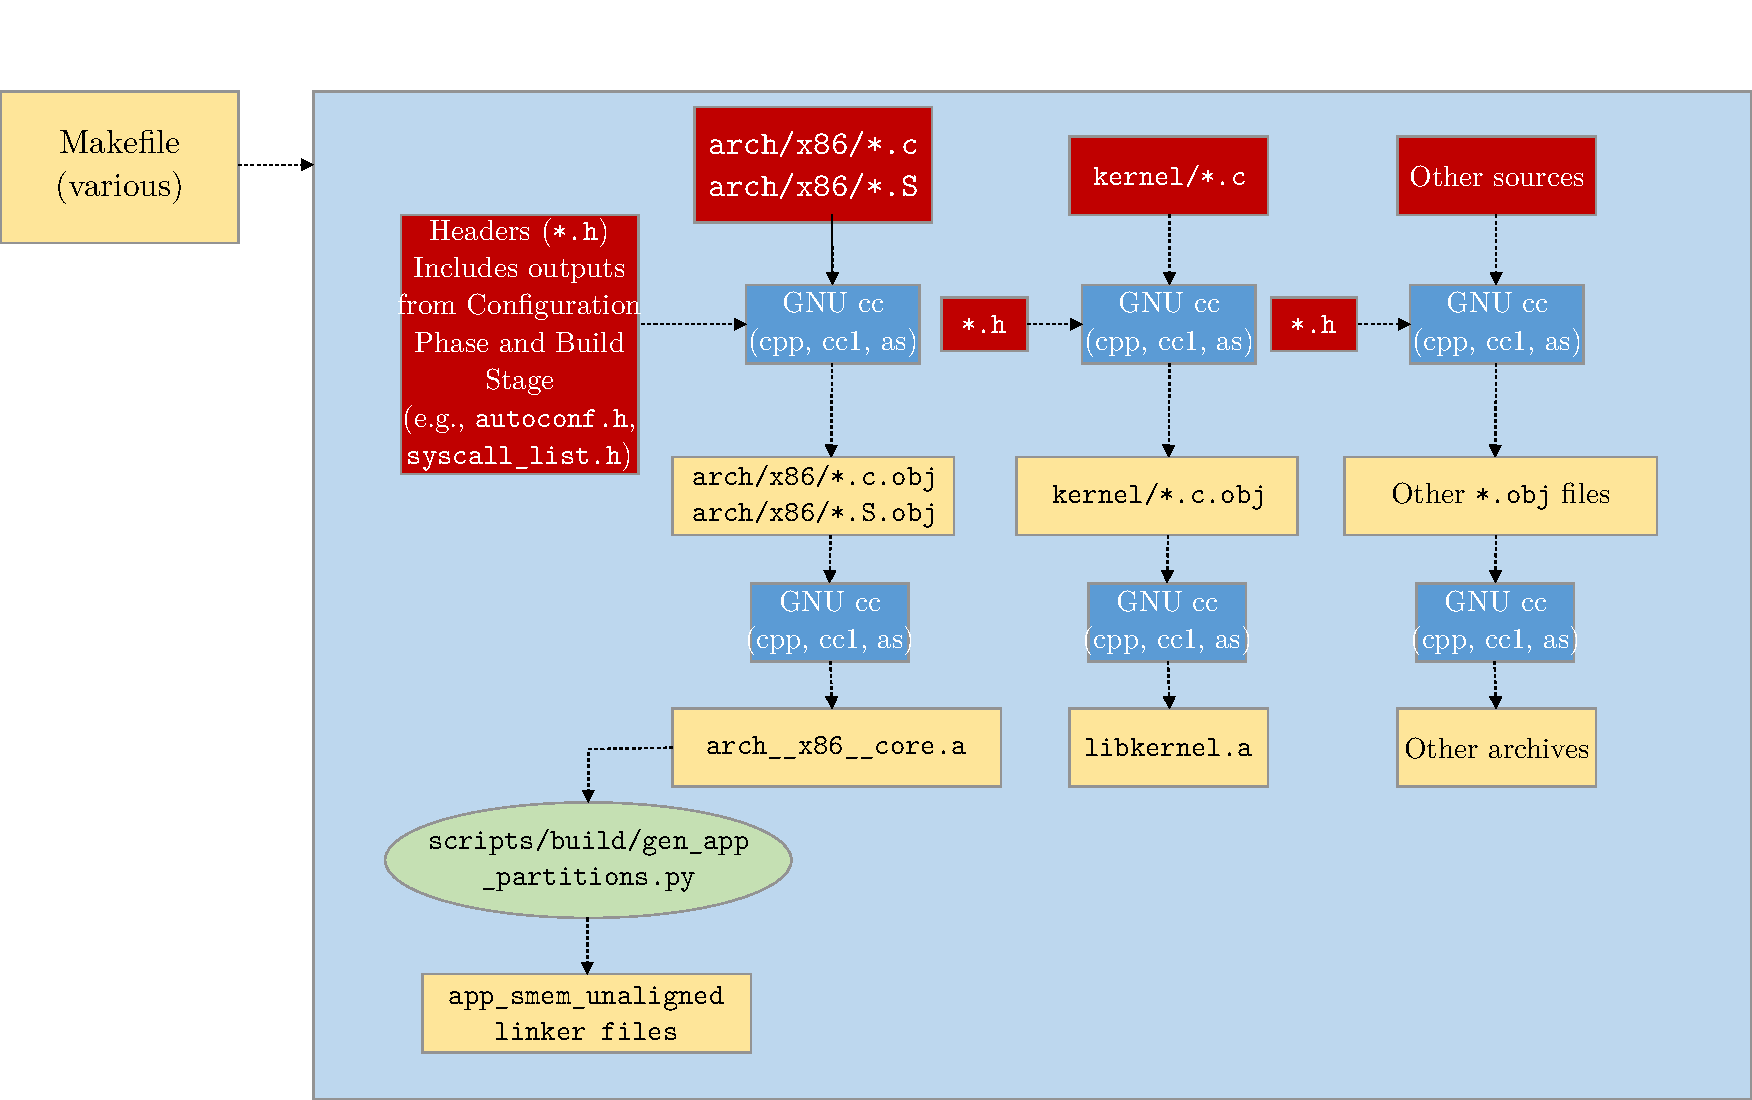
\includegraphics[width=\textwidth]{Figures/3_cmake_build2.pdf}
	\caption[Flowchart of ninja stage II, generation and compilation]{Flowchart of \texttt{ninja} build stage II, generation and compilation}
	\label{fig:3_build2}
\end{figure}
Next, in \cref{fig:3_build2} the build system collects source files for various subsystems (decided by the configuration phase) and compiles into archives. The \texttt{gen\_app\_partitions.py} script examines all the archives that are produced and creates linker scripts that organize and align application partitions correctly, based on the memory protection hardware of the target. Then \texttt{cpp} process involves merging linker script fragments from various sources, including the target's architecture/\gls{soc}, the kernel tree, partition output (if memory protection is enabled), and any other selected fragments from the configuration process. These are combined into a \texttt{linker.cmd} file. The compiled archives are then linked with \texttt{ld}, following the specifications in the \texttt{linker.cmd} file.
\begin{figure}[htbp]
	\centering
	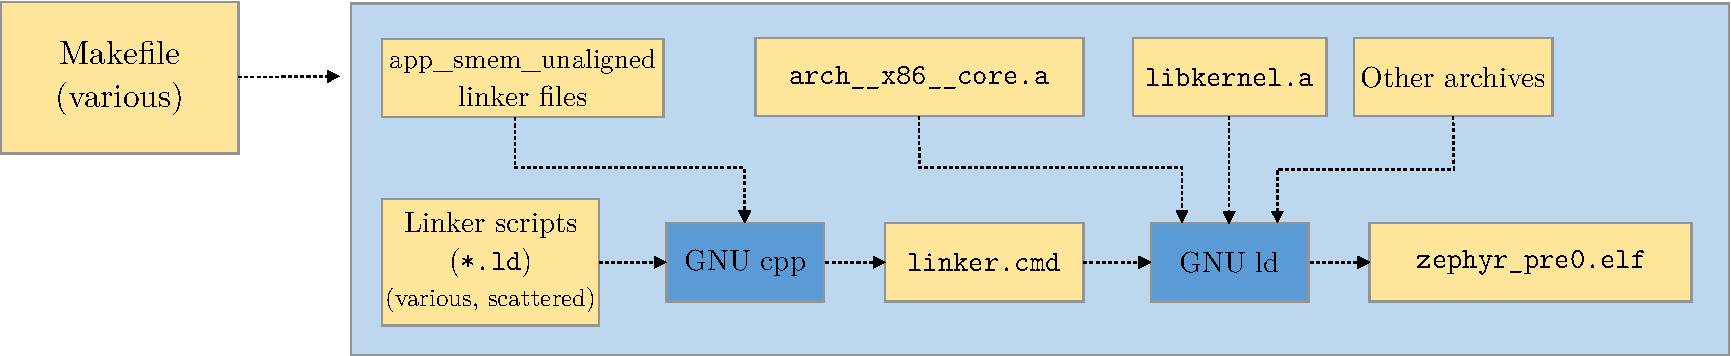
\includegraphics[width=\textwidth]{Figures/3_cmake_build3.pdf}
	\caption[Flowchart of ninja stage III, intermediate binary]{Flowchart of \texttt{ninja} build stage III, intermediate binary}
	\label{fig:3_build3}
\end{figure}
Shown in \cref{fig:3_build3} is the process, in which an unfixed size intermediate binary is produced. If a devicetree is being used, an intermediate binary is generated that has a variable size. The binary is not fixed in size, which means that it can be modified by post-processing steps that affect the size of the final binary.
\begin{figure}[htbp]
	\centering
	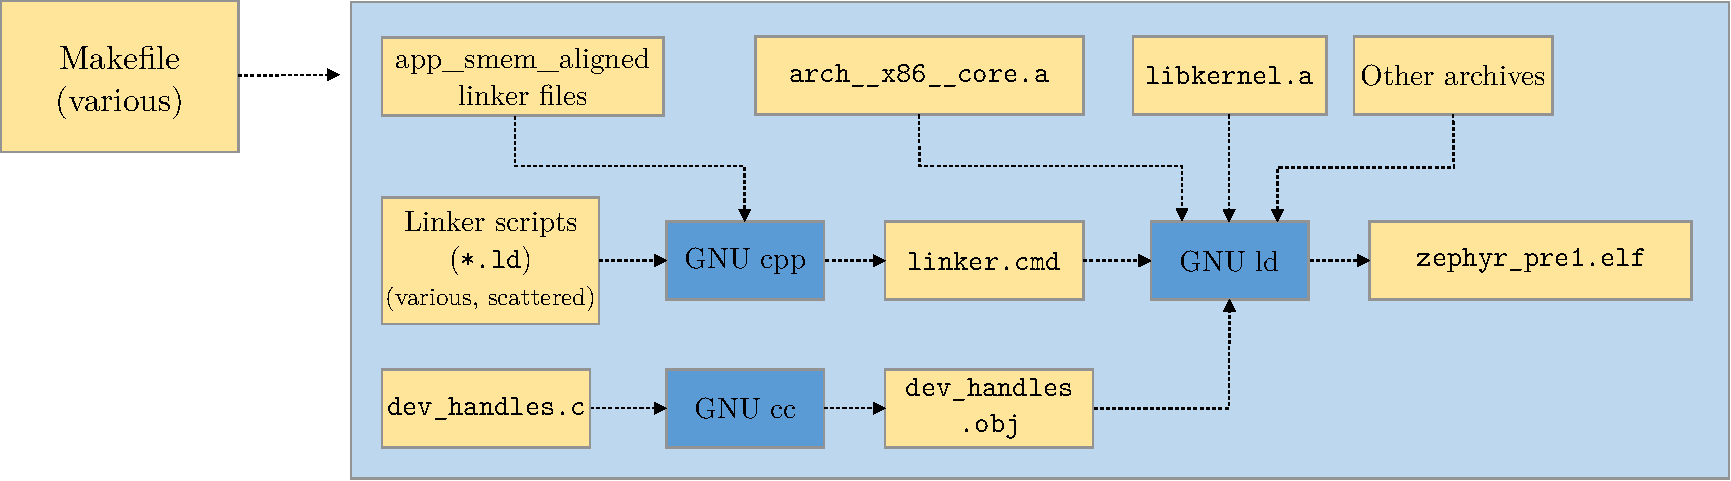
\includegraphics[width=\textwidth]{Figures/3_cmake_build4.pdf}
	\caption[Flowchart of ninja stage IV, second intermediate binary]{Flowchart of \texttt{ninja} build stage IV, second intermediate binary}
	\label{fig:3_build4}
\end{figure}
In \Cref{fig:3_build4} the fixed size intermediate binary is generated. The previous stage's binaries are not fully formed and contain sections that are empty or marked as placeholders. These sections must be filled in by a process similar to reflection. To finish building, certain scripts are run on the intermediate binaries. These scripts generate the necessary components that are missing from the final binary.
\begin{figure}[htbp]
	\centering
	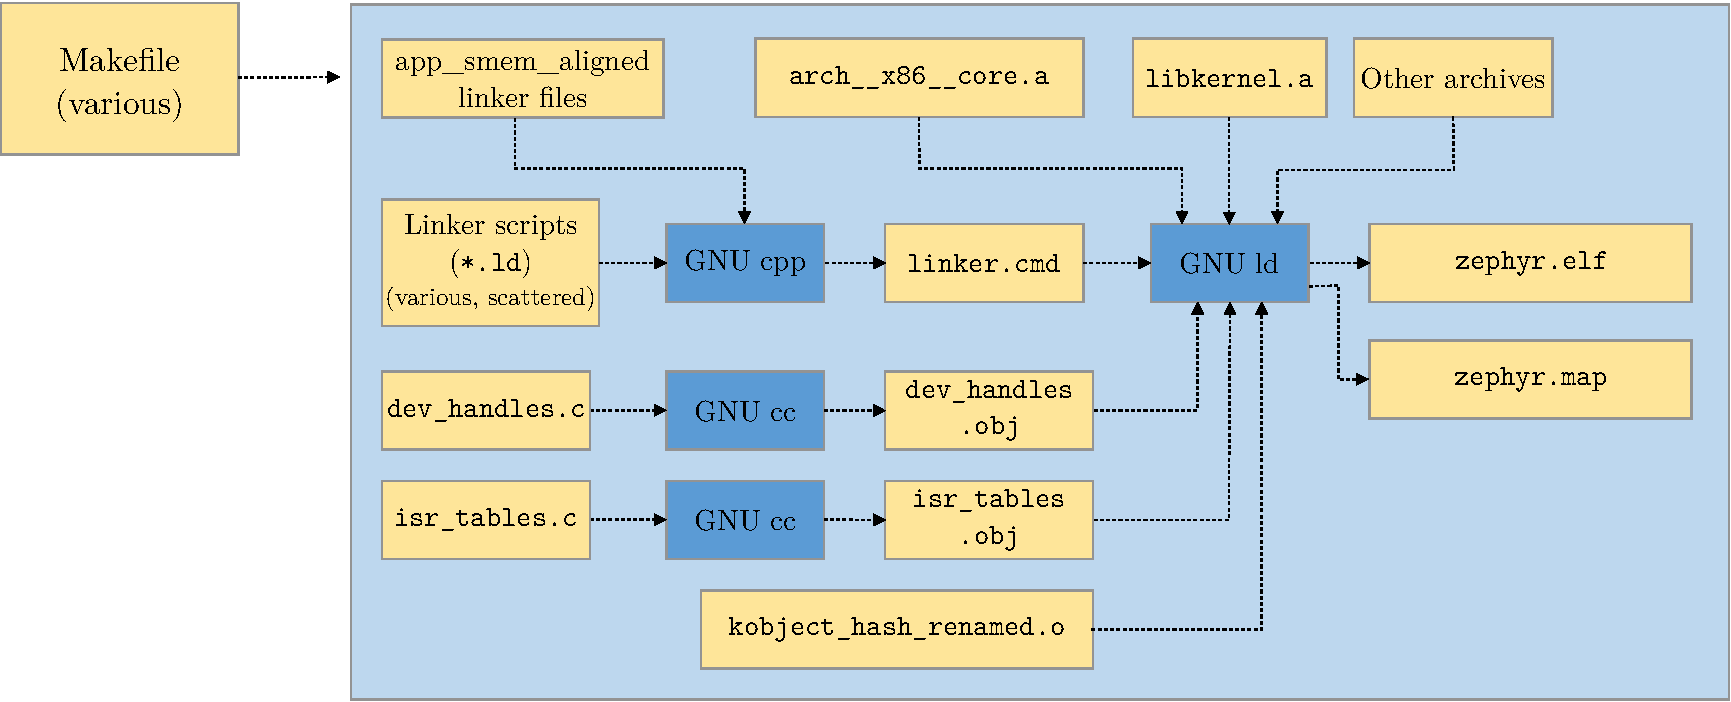
\includegraphics[width=\textwidth]{Figures/3_cmake_build5.pdf}
	\caption[Flowchart of ninja stage V, final binary]{Flowchart of \texttt{ninja} build stage V, final binary}
	\label{fig:3_build5}
\end{figure}
Next, in \cref{fig:3_build5}, the final binary is produced by repeating the link from the previous stage, but this time with all the missing pieces populated.
\begin{figure}[htbp]
	\centering
	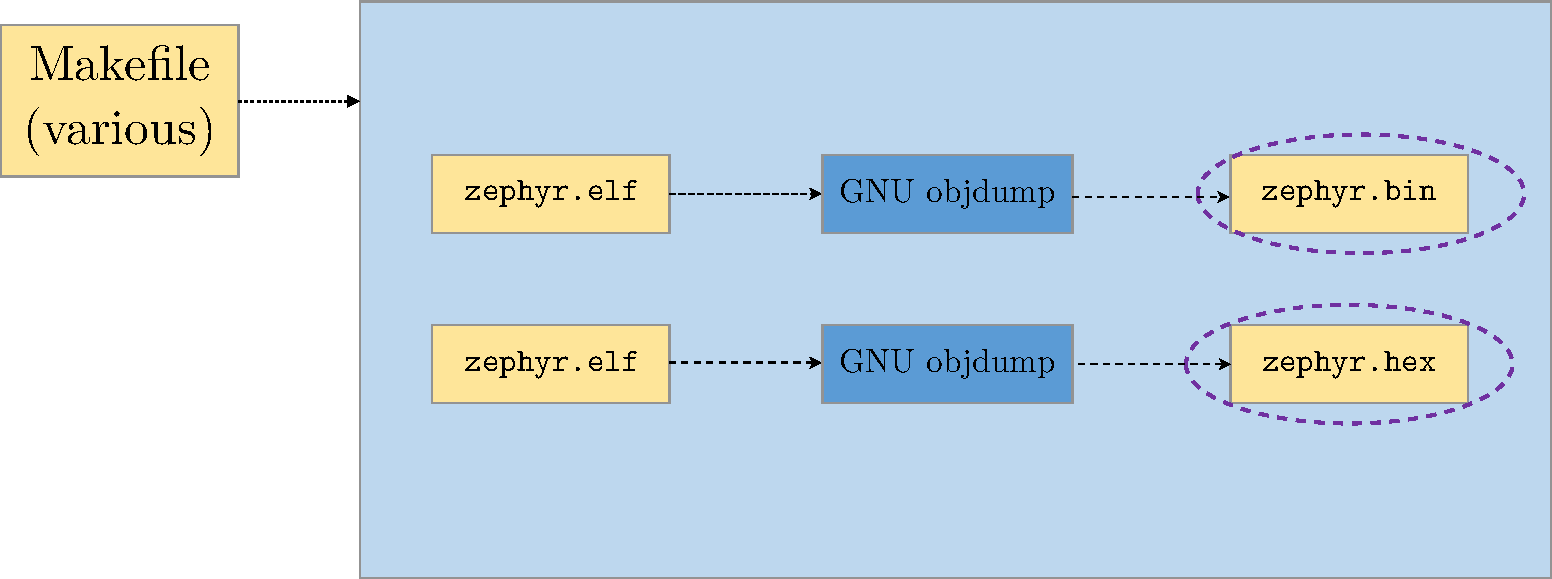
\includegraphics[width=.75\textwidth]{Figures/3_cmake_build6.pdf}
	\caption[Flowchart of ninja stage VI, final binary]{Flowchart of \texttt{ninja} build stage VI, post-processing}
	\label{fig:3_build6}
\end{figure}
Finally, using \texttt{GNU objdump}, the completed kernel is converted from a \gls{elf} file to the hex file that is expected by the flash tool compatible with the target device.

\section{Pulse-Width-Modulation Generator}
Initially, a waveform generator was designed by using a programmable synthesizer circuit, but due to constraints within generating dead-time when driving the half-bridge, a more accurate timer based PWM generation is required. In a half-bridge power stage, dead-time refers to the amount of time that elapses between the moment when one of the switches in the half-bridge (either the high-side or the low-side switch) turns off and the moment when the other switch turns on. During the dead-time, both switches in the half-bridge are off, which means that there is no current flowing through either switch in the half-bridge. A scenario where both switches are on, can cause problems if the output of the half-bridge is connected to a load, as it may cause the load to behave erratically or even be damaged. To avoid these problems, it is important to carefully consider the amount of dead-time in a half-bridge power stage. In general, a longer dead-time will reduce the risk of damage to the load, but it will also reduce the efficiency of the power stage, as energy will be lost during the dead-time. Therefore, it is important to carefully balance the trade-off between efficiency and safety in order to determine the optimal amount of dead-time for a given half-bridge power stage.
A complementary timer

\section{Power Stage}
\begin{figure}[htbp]
	\centering
	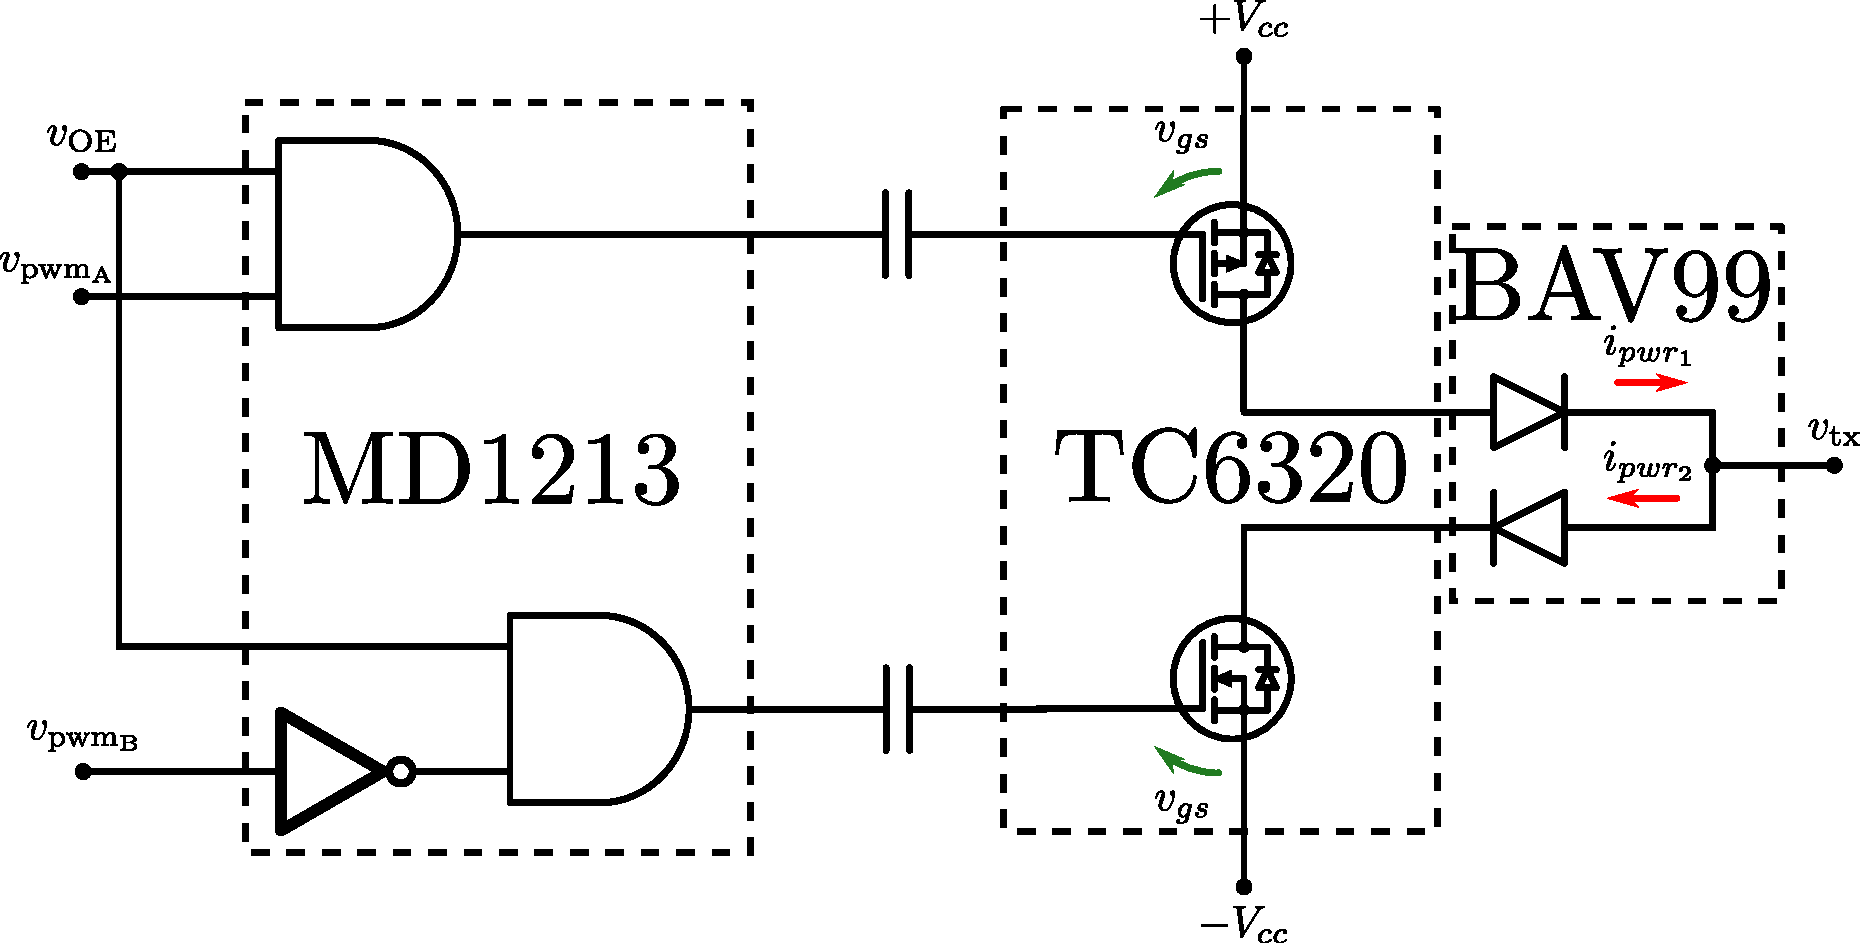
\includegraphics[width=\textwidth]{circuits/power_stage.pdf}
	\label{fig:3_power_stage}
	\caption{Circuit diagram of power stage}
\end{figure}
Gate drivers \cite{ISL55111,MD1213,EL7104}

\section{Transmit/Receive Switch}
\begin{figure}[htbp]
	\centering
	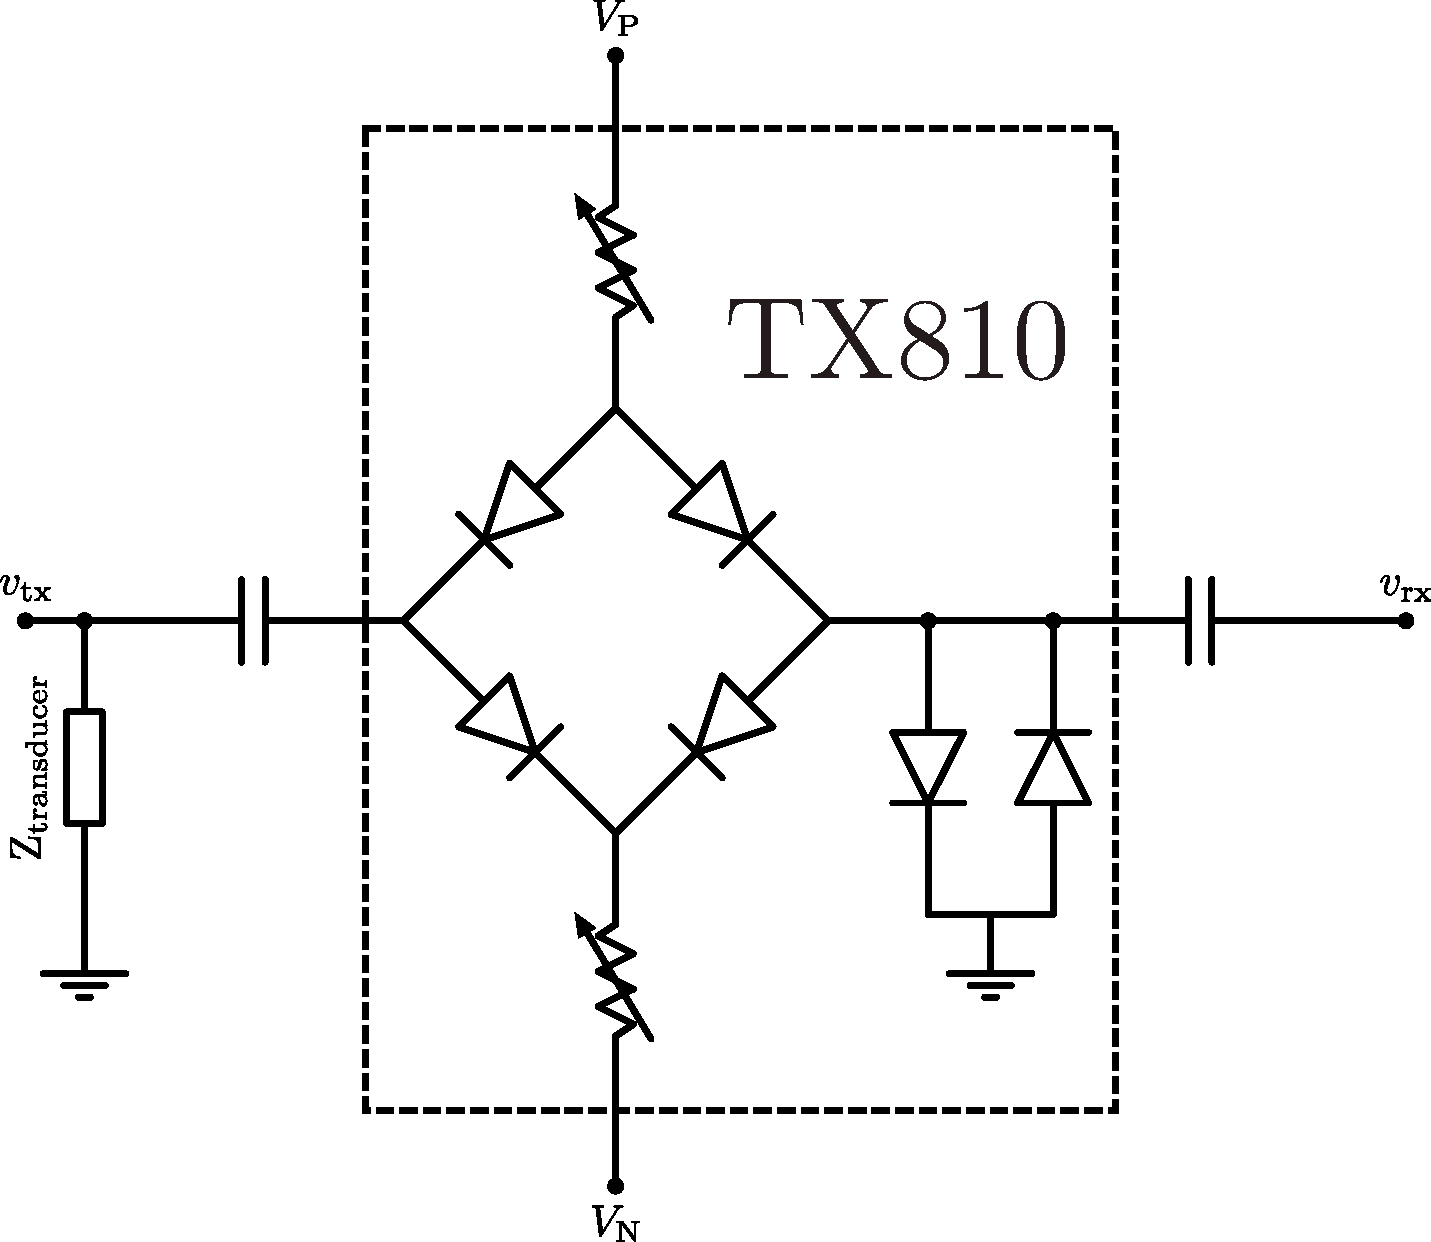
\includegraphics[width=.6\textwidth]{circuits/switch.pdf}
	\label{fig:3_switch}
	\caption{Circuit diagram of switch (per channel)}
\end{figure}
The transmit/receive switch is a module that is based on an IC from Texas Instruments known as TX810\cite{TX810}. The TX810 is an electronic device that can be used to switch transmit and receive paths of an ultrasound system. It can switch the transmit and receive paths for up to 8 different transducers (also known as probes) at the same time. The TX810 is programmed to switch the transmit and receive paths at specific times, as determined by the user. For example, the user can program the TX810 to switch the transmit and receive paths of a particular transducer at a specific time during the ultrasound examination. This allows the user to perform multi-channel imaging, where multiple transducers are used simultaneously to capture images from different angles. The IC is typically used in conjunction with an ultrasound system and one or more transducers. Transducers are used to transmit and receive ultrasound waves, which are used to generate images of the body's internal structures. The TX810 is used to switch the transmit and receive paths for each transducer at the appropriate times, allowing the ultrasound system to capture images from multiple angles simultaneously. When high-voltage transmitter signals are applied to the input, the internal diodes limit the output voltage. While in receive mode, the TX810's insertion loss is minimized. The TX810 features a 3-bit interface that may be used to program bias current from \qty{7}{\milli\ampere} to \qty{0}{\milli\ampere} for varying performance and power requirements, unlike conventional T/R switches. The device is put up in power-down mode when the TX810 bias current is set to 0mA (high-impedance mode). The TX810 does not put significant load on high-voltage transmitters when operating in the high-impedance mode. The device can also wake up from power-down mode in less than a \unit{\micro\second}. These sophisticated programmable features enable systems to save a large amount of electricity.

The module is designed with three channels available. That means three channels can be used, either three separate transducers for multi-angle sonography, or a \gls{cmut} with three channels in a single angle.

\section{Transducer}
Various \gls{transducer} types are used during the testing of this project. Initially, commercially available transducers were used in order to validate the experimental process of the pulse-echo and Doppler measurements. Commercially available transducers in this context means \gls{pzt} \gls{piezoelectric} transducers. PZT is a piezoelectric material that deforms when an electrical voltage is applied, and generates an electrical signal when it is mechanically deformed. PZT transducers are widely used for medical imaging due to their high piezoelectric efficiency, high bandwidth and durability.

At a later stage during the project, CMUTs are used. CMUT, is a newer technology that uses capacitance to convert between electrical and mechanical energy. The transducer consists of a flexible membrane that moves in response to an applied voltage, producing ultrasound signals. CMUTs have advantages in terms of their small size, high frequency, and ability to operate in a broad range of conditions, making them ideal for use in portable and high-resolution imaging devices. There are two types of CMUTs used:

\subsubsection{Rigid CMUTs:}
\begin{itemize}
	\item Advantages:
	\begin{itemize}
		\item Higher mechanical stability, leading to less noise and improved image quality
		\item Can handle higher pressures, making them suitable for deeper imaging applications
		\item Can have a larger surface area, providing higher sensitivity
	\end{itemize}
	\item Disadvantages:
	\begin{itemize}
		\item Less flexible, limiting their use in applications with complex geometries or limited access
		\item Higher stiffness, leading to increased power consumption and difficulty in producing high-frequency signals
	\end{itemize}
\end{itemize}
\subsubsection{Flexible CMUTs:}
\begin{itemize}
	\item Advantages:
	\begin{itemize}
		\item More flexible, allowing them to conform to complex geometries or be used in applications with limited access
		\item Can be made thinner and lighter, making them suitable for portable or handheld imaging devices
		\item Can be integrated into wearable devices or implanted into the body, enabling new imaging modalities
	\end{itemize}
	\item Disadvantages:
	\begin{itemize}
		\item Lower mechanical stability, leading to increased noise and reduced image quality
		\item Lower maximum operating pressure, limiting their use in deep imaging applications
		\item Smaller surface area, resulting in reduced sensitivity
	\end{itemize}
\end{itemize}
In summary, the choice between rigid and flexible CMUTs depends on the specific requirements of the application and the trade-off between flexibility, sensitivity, and image quality. For this project, a wearable transducer is desired and therefore the flexible CMUT is preferred.

\subsection{Impedance matching}
Impedance matching refers to the adjustment of the output impedance of the transducer to match the input impedance of the receiving system, such as the ultrasound machine or amplifier. This ensures maximum transfer of energy from the transducer to the receiving system, leading to improved signal strength and reduced noise in the final image. In ultrasound imaging, the transducer is used to both transmit and receive ultrasound signals. The impedance of the transducer must be carefully matched to the environment it is operating in, to ensure efficient transfer of energy both ways. If the impedance of the transducer and the receiving system do not match, a portion of the transmitted energy will be reflected back to the transducer, leading to reduced signal strength and increased noise in the final image. This can also result in increased power consumption and reduced battery life in portable or handheld imaging devices.

\section{Preamplifier}
\subsubsection{OPA487}
The OPA847\cite{OPA847} is a high-performance, high-speed, voltage feedback amplifier with a bandwidth of over \qty{1}{\giga\hertz}. It has a wide gain range, low distortion, and low noise, making it suitable for a variety of applications including video, RF, and high-speed data acquisition. The OPA847 has a single-ended input and a differential output, which allows it to be used in a variety of circuit configurations. It is available in a surface-mount package and operates over a wide supply voltage range.

\subsubsection{AD8332}
The AD8332\cite{AD8332} is a fully integrated, single-chip amplifier designed for use in a wide range of RF and microwave applications. It is a low-noise, high-linearity amplifier that can be used in a variety of configurations, including as a stand-alone amplifier or as part of a larger system. The AD8332 is a current-feedback amplifier that can operate over a wide frequency range, from \qty{50}{\mega\hertz} to \qty{4}{\giga\hertz}. It has a high level of integration, with all active components on a single monolithic IC. This makes it suitable for use in small form factor applications where space is at a premium. The AD8332 has a number of features that make it well-suited for use in RF and microwave applications. It has a high level of linearity, which allows it to amplify signals without introducing significant distortion. It also has a low noise figure, which makes it well-suited for use in low-noise applications. Additionally, the AD8332 has a wide \gls{dynamic range}, which makes it capable of handling a wide range of input signals without clipping or saturating. Overall, the AD8332 is a versatile and reliable amplifier that can be used in a wide range of RF and microwave applications. It is well-suited for use in a variety of systems, including communication systems, radar systems, and instrumentation systems.

\section{Demodulation}
To demodulate our signal using the process described in The AD8333\cite{AD8333} can be used to demodulate \gls{am} signals. It contains all the necessary circuitry to detect and extract the information contained in an AM signal. In AM, the information is encoded in the amplitude of the carrier wave, which is modulated or varied in some way to convey the information. The AD8333 is able to detect these variations in the carrier wave and extract the original information from the signal. To do this, the AD8333 uses a process called envelope detection. It rectifies the input signal, which removes the negative portions of the waveform, and then filters the resulting signal to remove any remaining high-frequency components. This leaves only the envelope of the original modulated signal, which contains the encoded information. The AD8333 also includes amplifier and buffer stages to amplify the detected envelope and prepare it for further processing or application. It is often used in radio communication systems, industrial control systems, and other applications where an AM signal needs to be demodulated and the information contained in the signal needs to be extracted. Test af git push.
\section{Sample/Hold}
The sample/hold circuit is based on the AD783\cite{AD783} \gls{sha}. It functions by converting an analog input signal into a sequence of \gls{quantized} samples and holds these samples for a specified time. The SHA is made up of several internal stages, including an input amplifier, sample switch, sample-and-hold capacitor, and output amplifier. When the sample input of the AD783 is triggered, the input amplifier amplifies the input signal and the sample switch closes, allowing the signal to be stored on the sample-and-hold capacitor. Once the sample is taken, the sample switch opens, and the output amplifier outputs the stored value of the input signal. The hold input of the AD783 maintains the sample on the capacitor until the next sample is taken.
\section{Pulse-Repetition and Wall Filter}

\section{Amplifier}

\section{Mixer}

\section{Adder}